%Start: 22/04/14
%Last edited on 17/09
	%Complete revision after committee meeting and NERD club
	%More straightforward story, clearer results with a more simple measure of diversity, took out the mandibles completely
	%Now aiming for the Journal of Mammalogy (needs very different formatting)


% Preamble
\documentclass[12pt,a4paper]{article}
\usepackage{enumerate} 	% put in numbers or bullet points
\usepackage{setspace}	% line spacing					
\usepackage{authblk}	% For author affiliations
\usepackage{graphicx} 	% For adding pictures

\usepackage[nomarkers]{endfloat} %Figures and tables at the end of the document
\usepackage{pdflscape}	% for landscape pages
\usepackage{mathtools}	% For equations etc.
\usepackage[osf]{mathpazo} % palatino font package
\usepackage{fixltx2e}	% includes subscripts
\usepackage{ms}     	% load the manuscript style template

%\usepackage{float}		% Use these options to have figures in specific places in the text
%\floatstyle{plaintop} 	% Force table captions to go above the table

\setcounter{secnumdepth}{0} % removes numbers from section headings
\raggedright 			% justify the text on the left only
\pagenumbering{arabic}	% Page numbers

%\onehalfspacing 		%1.5 line spacing - use the below instead in case you need double spacing for some journals
%\linespread{1.6} 		% this is 1.5 spacing, double line spacing is 1.6 - unrecognised command (maybe due to the setspace package?)
\usepackage[round]{natbib} % author-year citations in round brackets
%-----------------------------------------
%Title page
%----------------------------------------
\title{Morphological diversity of tenrec (Afrosoricida, Tenrecidae) skulls compared to their closest relatives, the golden moles (Afrosoricida, Chrysochloridae)} 
% I want to come up with a better title

\author{Sive Finlay$^{1,2,*}$ and Natalie Cooper$^{1,2}$}
\affiliation{\noindent{\footnotesize
$^1$ School of Natural Sciences, Trinity College Dublin, Dublin 2, Ireland.\\ 
$^2$ Trinity Centre for Biodiversity Research, Trinity College Dublin, Dublin 2, Ireland.\\
$^*$Corresponding author: sfinlay@tcd.ie; Zoology Building, Trinity College Dublin, Dublin 2, Ireland.\\ Fax: +353 1 6778094; Tel: +353 1 896 2571.\\}}
\date{}	% To give blank date

\runninghead{Cranial morphological diversity in tenrecs } %Need to fix this when I have a proper title

\keywords{geometric morphometrics, golden moles, morphological diversity, tenrecs}
%---------------------------------------------------------------
% Start of document
\begin{document}

\modulolinenumbers[1] 	% Line numbering on every line

\mstitlepage			% Instead of \maketitle you can use the nice template to get it looking like a manuscript
\parindent=1.5em		% Changes paragraph indenting so it's not so big
\addtolength{\parskip}{.3em} % Changes spacing between sections so it's smaller
%---------------------------------------------------
\begin{abstract} 

% Abstract need to be no more than 5 % of the rest of the text
	% Main message is the importance of quantitative vs. qualitative

	Morphologically diverse groups have long attracted the interest of biologists. Many studies now recognise the importance of quantifying patterns of morphological diversity to gain new insights into evolutionary patterns. Tenrecs (Afrosoricida, Tenrecidae) are a family of small mammals which is often cited as an example of an exceptionally morphologically diverse group. However, this assumption has not been tested. Here we use geometric morphometric analyses of skull shape to test whether tenrecs are more morphologically diverse than their closest relatives, the golden moles (Afrosoricida, Chrysochloridae). Contrary to our expectations, we find that tenrec skulls are only more morphologically diverse than golden moles when measured in lateral view. Furthermore, the similarities among the species-rich \textit{Microgale} tenrec Genus appear to mask higher morphological diversity in the rest of the Family. Our results reveal new insights into the morphological diversity of tenrecs and highlight the importance of using quantitative methods to test qualitative assumptions about patterns of morphological diversity.
	
\end{abstract}

\newpage
%-------------------------------------------------------
\section{Introduction} 

%1) Morphological diversity
	Morphological diversity has long attracted the attention of biologists.
% NC: This first sentence feels a bit disconnected from the following one. Could they be combined? Or could you lose the first sentence?
    There are many famous examples of exceptional morphological diversity including in the beaks of Darwin's finches, the body and limbs of Caribbean \textit{Anolis} lizards, and the pharyngeal jaws of cichlid fish \citep{Gavrilets2009}. %Or maybe find separate references for each one?
% NC: Probably want one reference each. Also, can you swap one for a mammal example for the paper since we are sending to J Mammal? I have also simplified
	Morphological diversity is important because it has implications for studies of adaptive radiations - where close relatives exhibit a range of divergent morphologies - \citep{Losos2010}, convergent evolution - where distant relatives exhibit similar morphologies - \citep[e.g.][]{Muschick2012, Harmon2005} and our understanding of biodiversity \citep{Roy1997}.
% NC: OK don't get the last one! How does it help? Our understanding of what exactly?
	However, apart from a few examples \citep[e.g.][]{Goswami2011, Ruta2013, Brusatte2008}, it is still common to study morphological diversity from a qualitative rather than quantitative perspective.

% NC: I switched the last two paragraphs as we need to know the general importance of diversity first, and then the problem i.e. it isn't quantified properly.

% NC: This probably needs a bit more finessing. 
	
%3) Difficult to measure (in general and back to tenrecs)
% NC: I switched these as I think you need more of the question before you get into specifics

	Morphological diversity is rarely studied from a quantitative perspective because it is difficult to quantify. Studies are inevitably constrained to measure the diversity of specific traits rather than overall morphologies \citep{Roy1997}. Different traits (such as cranial compared to limb morphologies) may yield different patterns of morphological diversity \citep{Foth2012}. %NC: Could you give a simple specific example? Just using two traits not suites of traits?
	Furthermore, linear measurements of morphological traits can restrict our understanding of overall morphological variation \citep{Rohlf1993} % NC: because...
	. Some of these problems can be solved by using geometric morphometric approaches \citep{Rohlf1993, Adams2013} that provide more detailed insights into morphological variation. Yet few studies have used these techniques to specifically address questions about morphological diversity in mammals.

%2) Tenrecs
% NC: Check out the changes I made (or didn't make!) to this section in your thesis intro!

	Tenrecs (Afrosoricida: Tenrecidae) are a morphologically diverse mammalian group \citep{Soarimalala2011, Olson2003}. The Family contains 34 species, 31 of which are endemic to Madagascar \citep{Olson2013}. Body sizes of tenrecs span three orders of magnitude (2.5 to $>$ 2,000g); a greater range than all other Families, and most Orders, of living mammals \citep{Olson2003}. Within this vast size range there are tenrecs which convergently resemble shrews (\textit{Microgale} tenrecs), moles (\textit{Oryzorictes} tenrecs) and hedgehogs (\textit{Echinops} and \textit{Setifer} tenrecs) \citep{Eisenberg1969} even though they are not closely related to these species \citep{Stanhope1998}. Despite these interesting features, the morphological diversity of tenrecs has never been properly quantified.

	% NC: Is this relevant? This is convergence. We are mainly just talking about tenrecs here

	%There are some qualitative similarities in the morphology of some tenrecs' limbs compared to other species \citep{Salton2009}. 

%4) Summary of findings
	Here we present the first quantitative investigation of morphological diversity in tenrecs. We use geometric morphometric approaches to compare cranial morphological diversity in tenrecs to their sister taxa, the golden moles (Afrosoricida, Chrysochloridae). 
	Tenrecs inhabit a wider variety of ecological niches than golden moles \citep{Soarimalala2011, Bronner1995} so we expect tenrecs to be more morphologically diverse. However, we only find a significant difference in the morphological diversity of skulls in lateral view, not dorsal or ventral. In contrast, when we restricted our data to include a subsample of the morphologically similar \textit{Microgale} tenrecs, we found that tenrecs were more morphologically diverse than golden moles in all three analyses.
	Our results highlight the importance of using quantitative methods to test assumptions about patterns of morphological diversity.
	%Needs a better last line here
	% NC: I think you still need to think carefully about the question you are trying to answer which may help with the last line. Also do you need to mention the complexity with different skull views here? Remember this is a very short summary of result. The real results will be in the abstract, results and discussion. Some journals don't even like you to include results in the intro. So short and simple is fine.

%-------------------------------------------------------------
\section{Materials and Methods}

	Our methods for measuring cranial morphological diversity involved several steps of data collection, processing and analysis. For clarity,  figure \ref{fig:flow} summarises all of these steps which are described in detail below.   
	
	%*************************************************
	%Methods flowchart
	%**************************************
		%landmarks diagram
		\begin{figure}
		\centering
		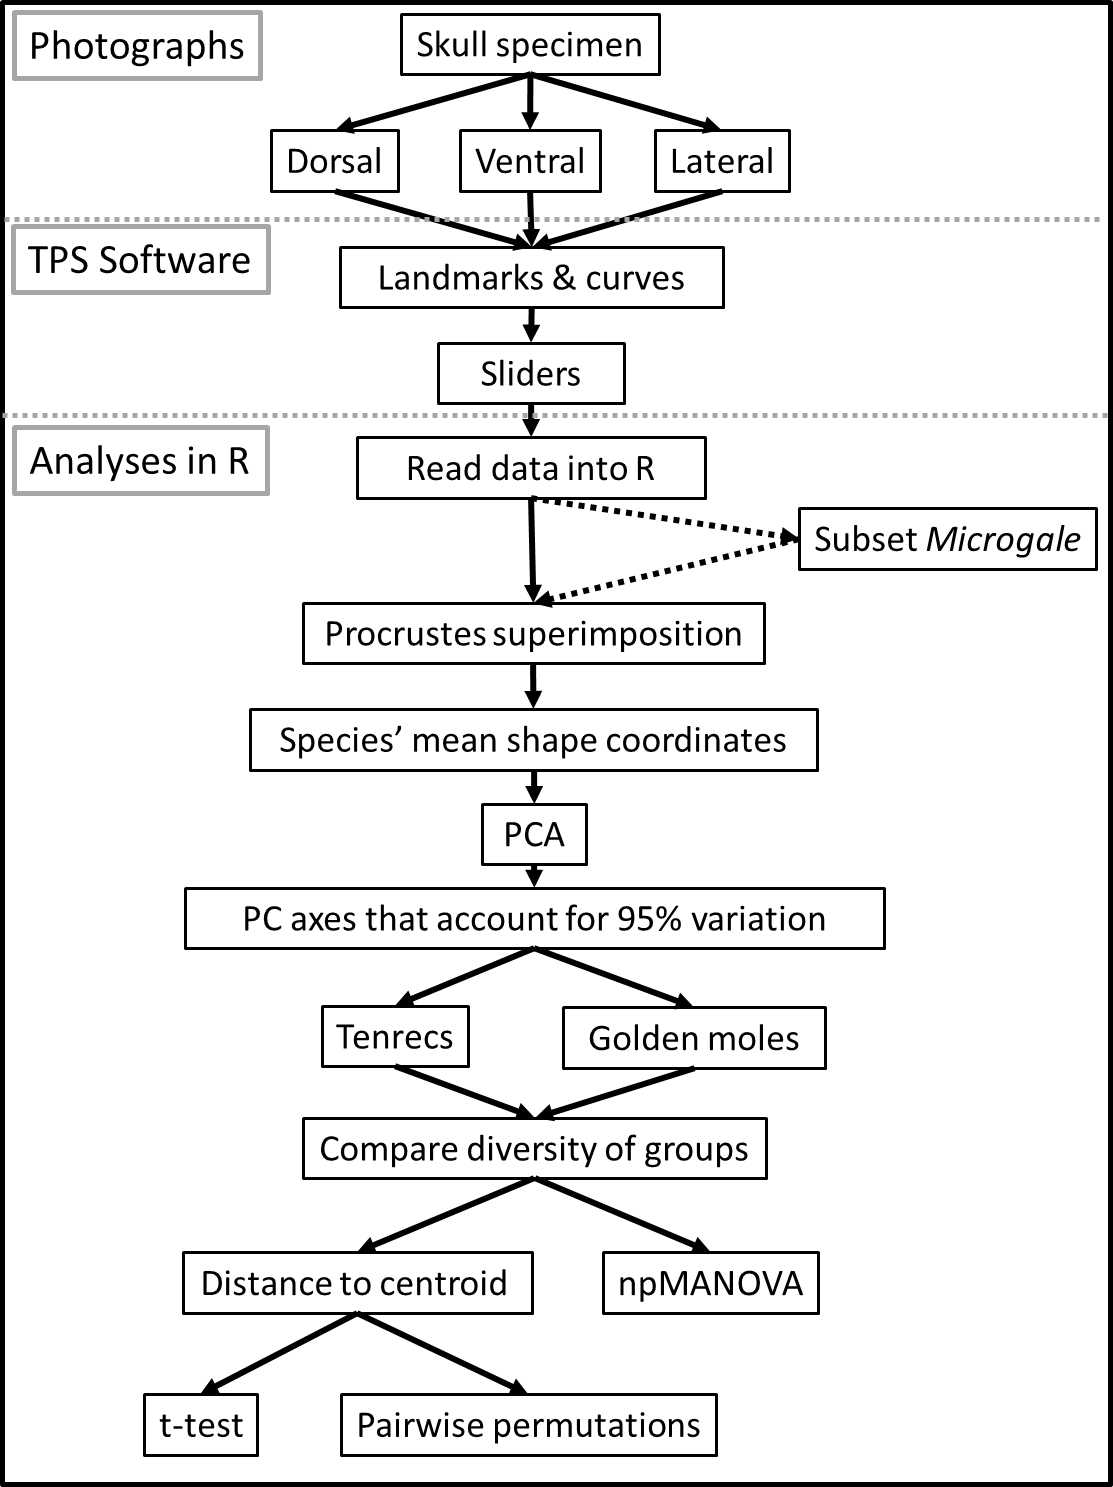
\includegraphics[width=1\linewidth]{figures/Methods_flowchart.png}
		
		\caption[Flowchart diagram of data collection and analysis]
			{Summary of the main steps in our data collection, processing and analysis protocol. Note that skulls were photographed in three views and the analyses were repeated separately for each view. The dashed arrows refer to the analyses we repeated including only a subset of \textit{Microgale} tenrecs.}
		
		\label{fig:flow}
		\end{figure}
	
	
	%************************************************** 

\subsection{Morphological data collection} % NC: Make sure to incorporate my edits from your thesis methods.
	
	One of us (SF) photographed crania of tenrecs and golden moles at the Natural History Museum London (BMNH), the Smithsonian Institute Natural History Museum (SI), the American Museum of Natural History (AMNH), Harvard's Museum of Comparative Zoology (MCZ) and the Field Museum of Natural History, Chicago (FMNH). We photographed the specimens with a Canon EOS 650D camera fitted with an EF 100mm f/2.8 Macro USM lens using a standardised procedure to minimise potential error (see supplementary material for details). 
		%SF: Remember my pictures are labelled NHML so I can just put a note with the figshare folder

	We collected pictures of the skulls in dorsal, ventral and lateral views (right side of the skull). A full list of museum accession numbers and details on how to access the images can be found in the supplementary material.
	
	
	%AMNH and SI pictures are on figshare but MCZ and FMNH are more tricky about copyright so I haven't put those pictures up
	% NC: May be worth linking to figshare here rather than just in suppl
	%Each of the picture sets have a different doi reference so I thought it might look clumsy to stick them in here. I've referred to each of them separately in the supplementary.

	In total we collected pictures from 182 skulls in dorsal view (148 tenrecs and 34 golden moles), 173 skulls in ventral view (141 tenrecs and 32 golden moles) and 171 skulls in lateral view (140 tenrecs and 31 golden moles) representing 31 species of tenrec (out of the total 34 in the family \citep{Olson2013}) and 12 species of golden moles (out of a total of 21 in the family \citep{Asher2010}). We used the taxonomy of Wilson and Reeder \citeyearpar{Wilson2005} supplemented with more recent sources \citep{Olson2013} to define our species. 
	

	We used a combination of landmarks (type 2 and type 3, \citep{Zelditch2012}) and semilandmarks to characterise the shapes of our specimens. Figure \ref{fig:skulls_landmarks} shows our landmarks (points) and semilandmarks (outline curves) for the skulls in each of the three views. Corresponding definitions of each of the landmarks can be found in the supplementary material.
	
	%semilandmark or semi-landmark? The Latter might improve readability
	%SF: it's usually semilandmark in other papers

	We used the TPS software series \citep{SUNY2009} to process and landmark the pictures (Fig. \ref{fig:flow}). We digitised all landmarks and semilandmarks in tpsDIG, version 2.17 \citep{Rohlf2013}. We re-sampled the outlines to the minimum number of evenly spaced semilandmark points required to represent each outline accurately \citep[][details in supplementary material]{MacLeod2013}. We used TPSUtil \citep{Rohlf2012} to create ``sliders'' files that defined which points in our TPS files should be treated as semilandmarks \citep{Zelditch2012}. We conducted all subsequent analyses in R version 3.0.2 \citep[][Fig. \ref{fig:flow}]{Team2014}. 
	
	We used the \texttt{gpagen} function in the \texttt{geomorph} package \citep{Adams2013} to run a general Procrustes alignment \citep{Rohlf1993} of the landmark coordinates while sliding the semilandmarks by minimising Procrustes distance \citep{Bookstein1997}. We used these Procrustes-aligned coordinates of all species to calculate average shape values for each species (n = 43) which we then used for a principal components analysis (PCA) with the \texttt{plotTangentSpace} function \citep{Adams2013}. 
	
	% NC: Use \texttt{} to make R functions and packages look like code.

	%Phylogenetic PCA of geometric morphometrics data doesn't affect distance-based morphological comparisons (identical results to normal PCA, Polly 2013). So I could put this in as a justification for using a normal rather than phylogenetic PCA approach?

% NC: Yep that's be a good idea.

%*************************************************
%Combined picture of three skull views
%**************************************
	%landmarks diagram
	\begin{figure}
	\centering
	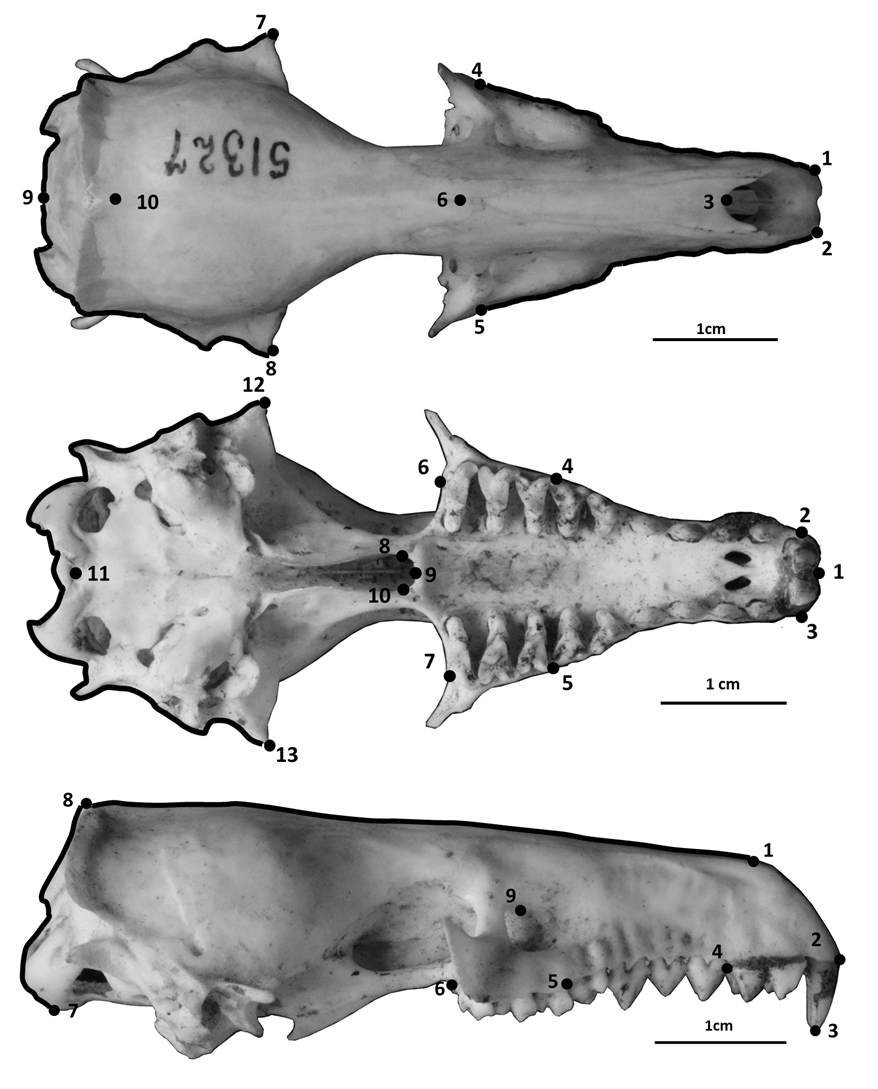
\includegraphics[width=1\linewidth]{figures/skdors+skvent+sklat_BW.png}
	
	\caption[Diagram of the landmarks and curves for the skulls in dorsal ventral and lateral views]
		{Landmarks (numbered points) and curves (black lines) used to capture the shape of skulls in dorsal, ventral and lateral views respectively. Curves were re-sampled to the same number of evenly-spaced points. See supplementary material for descriptions of the curves and landmarks. The specimens belong to two different \textit{Potamogale velox} (Tenrecidae) skulls: accession number AMNH 51327 (dorsal) and BMNH 1934.6.16.2 (ventral and lateral)}
	
	\label{fig:skulls_landmarks}
	\end{figure}


%************************************************** 

	
%-------------------------------------------------------	
\subsection{Calculating morphological diversity}

% NC: The below is pretty complicated. Being concise is good but this is really hard to follow (and I know what you did). Maybe consider simplifying and expanding in a few places. Not on the details, but in describing more clearly what you're talking about. I've called the cranial morphospace the "full" cranial morphospace. Could use "complete" instead. I think it makes it clearer. Consider adding diagrams, esp for thesis.

	We calculated morphological diversity using the results of our principal components analyses. We selected the principal components (PC) axes which accounted for 95\% of the cumulative variation for each of our three skull analyses. These axes represent the dimensions of our full cranial morphospace \citep{Polly2013}. 

	We used the scores from the PC axes to compare cranial morphologies in two ways (Fig. \ref{fig:flow}). First, we used non parametric MANOVAs %NC: Abbreviation - need to define
	\citep{Anderson2001} to test whether tenrecs and golden moles occupied significantly different positions within our full cranial morphospaces \citep[e.g][]{Serb2011, Ruta2013}. We then compared morphological diversity within tenrecs to the diversity within golden moles, defining morphological diversity as the mean Euclidean distance between each species and its Family centroid. %NC: Maybe have a diagram here?
	 If tenrecs are more morphologically diverse than golden moles, then they should be more dispersed within our full cranial morphospaces. % NC: Not sure you need this - you've already said what you're comparing and it'll be obvious you used a ttest from the results. %We used a t-test to assess whether there was any significant difference in the morphological diversity (spread in morphospace) of tenrecs and golden moles.
	
	Our groups have unequal sample sizes (31 tenrec species compared to 12 golden mole species). Morphological diversity is usually decoupled from taxonomic diversity \citep[e.g.][]{Ruta2013, Hopkins2013} so larger groups are not necessarily more morphologically diverse. However, comparing morphological diversity in tenrecs to the diversity of a smaller Family could still bias our results. To account for this, we used pairwise permutation tests as follows. 
	
	We assigned each species to either ``tenrecs'' or ``golden moles'' at random and then calculated the difference in morphological diversity for the new groupings as described above. We repeated this procedure 1000 times to generate a null distribution of the expected differences in morphological diversity between a group with 31 members (``tenrecs'') compared to one with 12 members (``golden moles''). If there is no difference between the morphological diversity of tenrecs and golden moles, then the group identity (``tenrec'' or ``golden mole'') of each species is arbitrary, %i.e. if you randomly assign the species as being either a tenrec or golden mole and then re-calculate morphological diversity there would still be no difference in the diversity of the two groups. 

	Finally, we compared our observed measures of the differences in morphological diversity between the two Families to our null distributions to determine whether there were significant differences after taking sample size into account.

% NC: I'm confused - I see how the permutations give you a p value, but how do they account for sample size? And are they being used to get p values? If so why isn't that mentioned? 
	
	The majority of tenrec species (19 out of 31 in our dataset) belong to the \textit{Microgale} (shrew-like) Genus that has relatively low morphological diversity \citep{Soarimalala2011, Jenkins2003}. This may mask signals of higher morphological diversity among other tenrecs. 
	To test this, we created a subset of our tenrec data that included just five of the \textit{Microgale} species, each representing one of the five sub-divisions of \textit{Microgale} outlined by Soarimalala and Goodman \citeyearpar{Soarimalala2011}, i.e. small, small-medium, medium, large and long-tailed species. We compared the morphological diversity of this subset of tenrecs (n=19: five \textit{Microgale} and 12 non \textit{Microgale} species) to that of golden moles using the methods described above (Fig. \ref{fig:flow}).
	 
% NC: Now this is shortened I'd stick the rarefaction in here too
	% SF: I took out rarefaction because Steve Wang and Steve Brusatte both advised that it was not the most appropriate test to use. The permutation method also takes sample size into account so I thought that removed the need for a rarefaction analysis aswell?

% NC: I'm currently really confused how the permutation removes the effects of sample size. Do you understand? If so try and explain it more clearly above.
%-----------------------------------------------------------

\section{Results}
 
	%New axes numbers (select axes for 95 % of the variation, not one extra)
		%Full data: skdors =6, skvent=7, sklat =7
		%Microgale subset: skdors=6, skvent=6, sklat=6
	Figure \ref{fig:sklatPCA} depicts the morphospace plot 
	% NC: Bit confusing here. It's not the whole morphospace, it's just PC1 and 2. Also in fig legend need to write out principal components somewhere as they should be understood independent of the text
	derived from our principal components analysis of average Procrustes-superimposed shape coordinates for skulls in lateral view. Similar plots for our analyses of skulls in dorsal and ventral views can be found in the supplementary material.
	To compare morphological diversity in the two families, we used the principal components axes which accounted for 95\% of the cumulative variation in each of our skull analyses: dorsal (n=6 axes), ventral (n=7 axes) and lateral (n=7 axes). 
	
	First, we compared the position of each Family within the morphospace plots. Tenrecs and golden moles occupy significantly different positions in the dorsal 	(npMANOVA, F \textsubscript{1,42} = 68.13, R$^2$ = 0.62, p=0.001 ), ventral (npMANOVA, F \textsubscript{1,42} = 103.33, R$^2$ = 0.72 , p=0.001 ) and lateral (npMANOVA, F \textsubscript{1,42} = 76.7, R$^2$=0.652, p=0.001 ) skull morphospaces,  indicating that the Families have very different, non-overlapping cranial morphologies. 
	
	%Numbers are from the npMANOVA based on PC axes within my diversity_twofamily_cent_dist script

	Secondly, we compared the morphological diversity within each Family. Based on our measures of mean Euclidean distance to the Family's centroid, tenrec skulls are more morphologically diverse than golden mole skulls when they are measured in lateral view but not in dorsal or ventral view (table \ref{tab:diversity}). In contrast, when we compared morphological diversity within the sub-sample of 19 tenrecs (including just five \textit{Microgale} species) to the 12 golden mole species, we found that tenrecs had significantly higher morphological diversity than golden moles in all analyses (table \ref{tab:diversity}).

	Our pairwise permutation tests for each analysis confirmed that differences in morphological diversity were not artefacts of differences in sample size (see supplementary material).
		%Add the new permutation results to the supplementary
%************************************
%Results tables and figures
%Reduced it down to one table and one figure

%This table is very squashed so I could break it up into two?
% NC: Could have two stacked on top of each other and then put the number of tenrec species as an extra column?
% NC: Also why are SE in brackets? In column headings mean and se are in brackets. I'd remove the brackets!
	\begin{table}[h]			
	\caption[Comparison of morphological diversity in tenrecs and golden moles.]
	\centering{Morphological diversity in tenrecs and golden moles for each of the three analyses (skulls in dorsal, ventral and lateral view). Results are shown for all 31 species of tenrec (left) and 19 species of tenrec (right) including just five \textit{Microgale} species. Significant differences (p $<$ 0.05) are highlighted in bold.}
	%Diversity based on centroid distances results summary
%All tenrecs and golden moles
%Morphological diversity based on comparing the mean Euclidean distances to each family's centroid
%NB: degrees of freedom are different in each analysis because I'm using a Welch two sample t test: df comes from a distribution of values based on the error within each sample so the final numbers will be different for each data set

%Re-ordered the table so that everything would fit in better


\resizebox{\columnwidth}{!}{
%Scales down the table to fit within the column width
	% If this is too small then I'll probably need to break the table into two
\begin{tabular}{c l c c c c}		
\hline
N& Analysis & \multicolumn{2}{c}{Morphological diversity} & t\textsubscript{df} & p value\\
%-----------------------------------------------
\hline
%------------------------
 &  & Tenrecs  & Golden moles &  &  \\
%--------------------------------
\cline{3-4} % Puts a line just through some columns
%---------------------------------
 & & (mean $\pm$ s.e) & (mean $\pm$ s.e) & &\\
\hline
%\multicolumn{1}{l}
%---------------------------
 31 & Skulls dorsal & \multicolumn{1}{l}{0.036 $\pm$ 0.0029} & 0.029 $\pm$ 0.0032 & -1.63\textsubscript{29.88}& 0.11 \\
%--------------------------------------
 & Skulls ventral & \multicolumn{1}{l}{0.048 $\pm$ 0.0034} & 0.044 $\pm$ 0.0041 & -0.68\textsubscript{26.99} & 0.51\\
%-----------------------------------------
 & Skulls lateral & 0.044 $\pm$ 0.0041 & 0.032 $\pm$ 0.0037 & -2.16\textsubscript{35.03} & \textbf{0.04}\\
%----------------------------------------
 & Mandibles & 0.049 $\pm$ 0.0044 & 0.067 $\pm$ 0.0054 & 2.62\textsubscript{25.85} & \textbf{0.01}\\
%--------------------------
\hline
%-----------------------------------------
17 & Skulls dorsal & 0.044 $\pm$ 0.0025 & \multicolumn{1}{l}{0.029 $\pm$ 0.0032} & -3.62\textsubscript{22.75} & \textbf{<0.01}\\
%---------------------------------
 & Skulls ventral & \multicolumn{1}{l}{0.054 $\pm$ 0.0039} & \multicolumn{1}{l}{0.042 $\pm$ 0.0041} & -2.23\textsubscript{25.46} & \textbf{0.04}\\
%-------------------------------------
 & Skulls lateral &  \multicolumn{1}{l}{0.054 $\pm$ 0.0053} & 0.031 $\pm$ 0.0037 & -3.47\textsubscript{26.31} & \textbf{<0.01} \\
%--------------------
 & Mandibles & 0.055 $\pm$ 0.0049 & \multicolumn{1}{l}{0.062 $\pm$ 0.0050} & 1.00\textsubscript{25.88} & 0.33 \\
%--------------------

\hline
\end{tabular}
} 
	\label{tab:diversity}  
	\end{table}

		
%PCA figure: Just sklat as an example
	%From the diversity_twofamily_cent_dist script
	\begin{figure}[H]
	\centering
	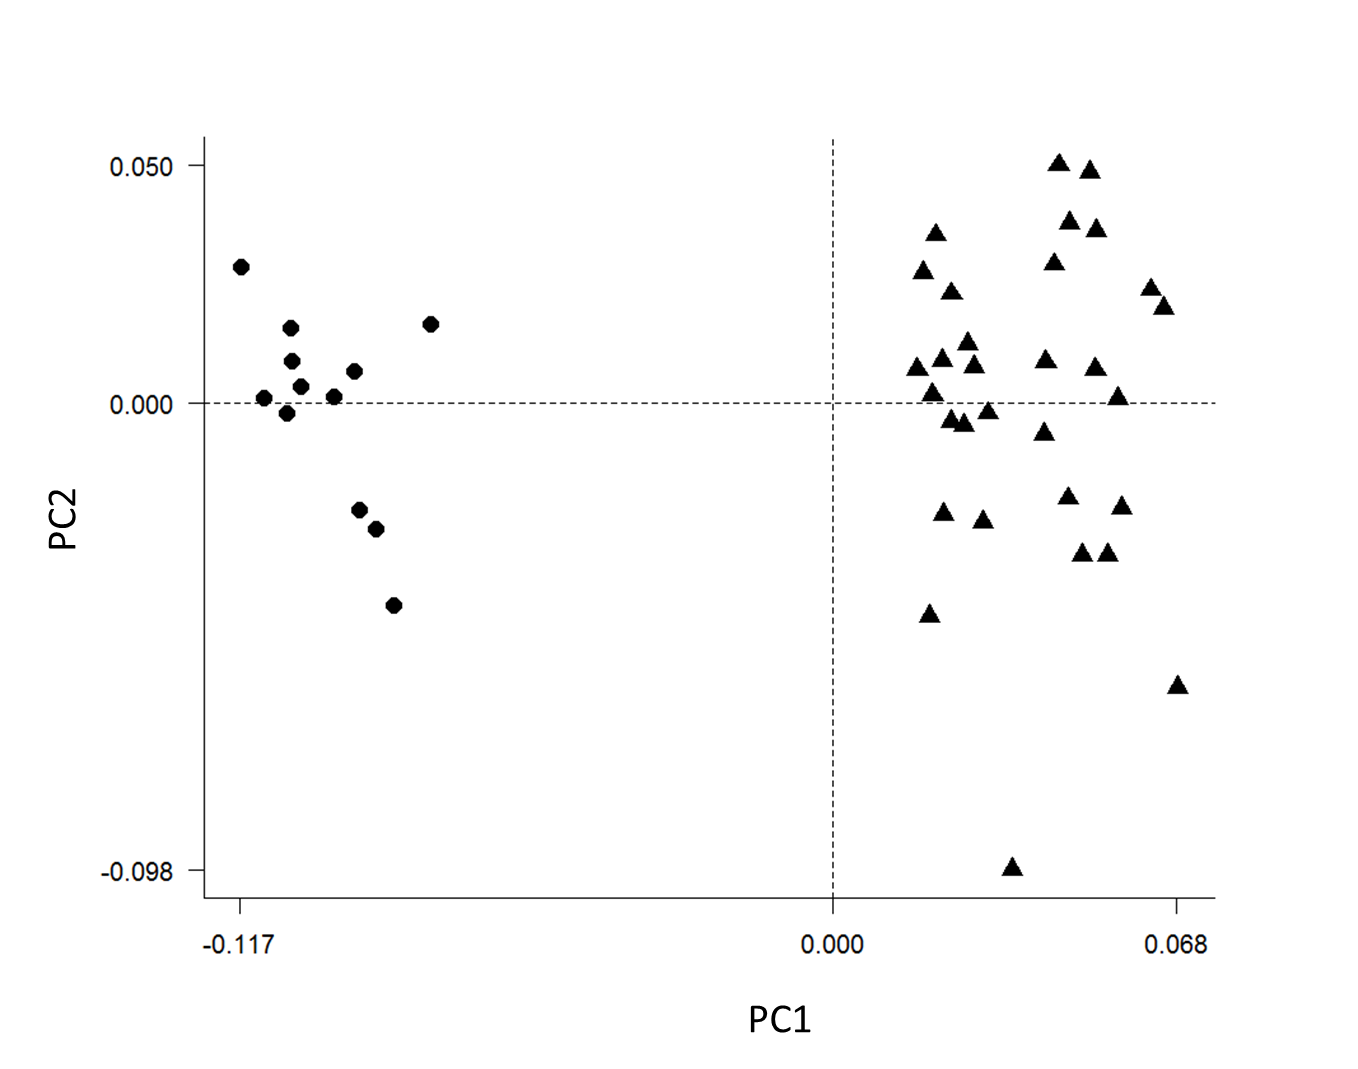
\includegraphics[width=1\linewidth]{figures/sklat_PCA_allspecies_BW.png}
	\caption[Morphospace (principal components) plot of morphological diversity in lateral views of tenrec and golden mole skulls.]
		{Principal components plot of the morphospace occupied by tenrecs (triangles, n = 31 species) and golden moles (circles, n = 12) for the skulls in lateral view. Each point represents the average skull shape of an individual species. Axes are PC1 and PC2 of the average scores from a PCA analysis of mean Procrustes shape coordinates for each species.}
	\label{fig:sklatPCA}
	\end{figure}
%**********************************************


\section{Discussion} 

%1) Results: strange and why 
	Tenrecs (Tenrecidae) are often cited as an example of a mammalian group with high morphological diversity \citep{Olson2013, Soarimalala2011, Eisenberg1969} and we expected them to be more morphologically diverse than their closest relatives the golden moles (latin name!). However, tenrecs were only more morphologically diverse than golden moles in one of our three skull analyses (lateral view; table\ref{tab:diversity}). Furthermore, the morphologically similar \textit{Microgale} tenrecs seem to mask high morphological diversity in the rest of the tenrec Family; reducing our data to include a sub-sample of this \textit{Microgale} species revealed that the remaining tenrecs were significantly more morphologically diverse than golden moles across all three skull analyses (table \ref{tab:diversity}). % NC: This is more a conclusion than a result so I've moved it to the end of the paragraph
	These results highlight the importance of using quantitative methods to test qualitative assumptions about patterns of morphological diversity.
	
%2) Why are lateral skulls different
	In our full analyses, tenrecs only had higher morphological diversity than golden moles when the skulls were measured in lateral view. This is most likely due to our choice of landmarks. The two outline curves in lateral view (Fig. \ref{fig:skulls_landmarks}) emphasise morphological variation in the back and top of the skulls, indicating that tenrecs are more morphologically diverse than golden moles in their three dimensional height. %NC: What is 3D height???
	These lateral aspects of the skull morphology could not be included in the dorsal and ventral analyses. In contrast, our landmarks in the dorsal, and particularly ventral, views focus on morphological variation in the overall outline shape of the skull and palate (Fig. \ref{fig:skulls_landmarks}). The result that tenrecs are no more diverse than golden moles in these areas makes intuitive sense: most tenrecs have broad, non-specialised diets \citep{Olson2013} so there is no obvious functional reason why they should have significantly diverse palate morphologies.
	Therefore, comparing the morphologies in three separate views allowed us to identify the more morphologically variable skull regions. 
	
	%Another sentence here about the importance of taking different 2D aspects for geometric morphometrics of a 3D object?

	%NC: Yeah *if* you'd have got a different result using linear measurements. But would you have? 
	
	
%3) Why does sub-sampling the Microgale make a difference?
	Measures of morphological variation are sensitive to the sampling used. If a particular morphotype is over-represented then the similarities among those species will reduce the overall morphological variation within the group \citep{Foote1991}. This appears to be the case for our data: it is only when we included a sub-sample of \textit{Microgale} tenrecs that we found higher morphological diversity in tenrecs compared to golden moles across all three skull analyses (table \ref{tab:diversity}). These results indicate that the overall morphological diversity within tenrecs is not as large as is often assumed \citep[e.g.][]{Eisenberg1969, Olson2013} because the majority of the Family are members of a single, morphologically similar Genus.

%4) Difficulties and caveats: body size, trait choice, morphological proxy

	Of course our results are based on a single morphological axis; the diversity of skull shape. It is difficult to quantify overall morphological diversity because any study is inevitably constrained by its choice of specific traits \citep{Roy1997}. Many other studies have also used skulls to study morphological variation within species \citep{Blagojevic2011, Bornholdt2008}, to delineate species boundaries within a clade \citep[e.g.][]{Panchetti2008} or for cross-taxonomic comparative studies of morphological (dis)similarities \citep[e.g.][]{Ruta2013, Goswami2011, Wroe2007}. 
	However, variation in skull shape is only one aspect of overall morphology. Quantifying variation in other morphological traits could yield different patterns. Therefore future work should extend our approach beyond just skulls to gain a more complete understanding of the overall morphological diversity of tenrecs and golden moles. 
		
%5) Conclusions
	We have presented the first quantitative investigation of morphological diversity in tenrecs. We found that tenrec skulls are more morphologically diverse than their closest relatives the golden moles, but only in some aspects of their morphology. Furthermore, our results indicate that the similarities among the species rich \textit{Microgale} tenrecs mask signals of higher morphological diversity among the rest of the Family. Of course our results are restricted to just one axis of morphological variation and further analysis of other traits is required. However, our results represent a significant step towards a more quantitative understanding of patterns of morphological diversity in tenrecs. 


%---------------------------------------------------	
 
	
\section{Acknowledgments}

	We thank Fran\c{c}ois Gould, Dean Adams, David Polly, Gary Bronner, Steve Brusatte, Steve Wang, Luke Harmon, Thomas Guillerme and the members of NERD club for insightful discussions and museum staff and curators % NC: Should probably name people who you worked with - they may get this to review. So mention the collections managers who let you in basically - so Steve, Louise that nice lady at the SI...
	for their support and access to collections. Funding was provided by an Irish Research Council EMBARK Initiative Postgraduate Scholarship (SF) and the European Commission CORDIS Seventh Framework Programme (FP7) Marie Curie CIG grant. Proposal number: 321696 (NC)

\bibliographystyle{jeb}
\bibliography{refs_disparity}
% I downloaded the jeb.bst file from http://schneider.ncifcrf.gov/latex.html but there isn't an associated style file

% NC: You can make one via the command line as I showed you in one of my LaTeX lessons.

	%**********************
	%SF: I still need to do this so that the references have the abbreviated journal titles, don't include the doi and so that book references don't have the total number of pages but do have the editors' names
	%*******************************************




\end{document}